%%%%%%%%%%%%%%%%%%%%%%%%%%%%%%%%%%%%%%%%%%%%%%%%%
%%%%%  make IFJtalk13.pdf
%%%%%%%%%%%%%%%%%%%%%%%%%%%%%%%%%%%%%%%%%%%%%%%%%
\documentclass{beamer}
%\documentclass[handout]{beamer}


\mode<presentation>
{
  \usetheme{Warsaw}
 %\usetheme{Hannover}
  \setbeamercovered{transparent}
}

\usepackage[english]{babel}
\usepackage{xcolor}
\usepackage[latin1]{inputenc}

\usepackage{times}
\usepackage[T1]{fontenc}
\usepackage{listings}
%------------------------------------------------------
\usepackage{amsbsy}
\usepackage{amsmath,amssymb,bbm}
\usepackage{euscript}
\usepackage{fancybox}


%%%%%%%%%%%%%%%%%%%%%%%%%%%%%%%%%%%%%%%%%%%%%%%%%%%%%%%%%%%%%%%
%%% Macros 
\newcommand{\Pcal}{{\cal P}}
\newcommand{\Kcal}{{\cal K}}
\newcommand{\Dcal}{{\cal D}}
%
\newcommand{\Peu}{\EuScript{P}}
\newcommand{\Keu}{\EuScript{K}}
\newcommand{\Deu}{\EuScript{D}}
\newcommand{\Reu}{\EuScript{R}}
\newcommand{\Feu}{\EuScript{F}}
%
\newcommand{\Pmf}{\mathfrak{P}}
\newcommand{\Dmf}{\mathfrak{D}}
%
\newcommand{\Pbbm}{\mathbbm{P}}
\newcommand{\Rbbm}{\mathbbm{R}}
\newcommand{\Zbbm}{\mathbbm{Z}}
\newcommand{\Bbbm}{\mathbbm{B}}
\newcommand{\Pop}{\overleftarrow{\Pbbm}}
\newcommand{\Zop}{\overleftarrow{\Zbbm}}
\newcommand{\Bop}{\overleftarrow{\Bbbm}}
\newcommand{\Rop}{\overleftarrow{\Rbbm}}
%
\newcommand{\Tbf}{\mathbf{T}}
\newcommand{\Pbf}{\mathbf{P}}
\newcommand{\Dbf}{\mathbf{D}}
\newcommand{\Phibf}{\mathbf{\Phi}}
%
\newcommand{\udl}{\underline}
\newcommand{\from}{\leftarrow}
\newcommand{\bu}{\bullet}
\newcommand{\veps}{\varepsilon}
\newcommand{\Dyfs}{D_{_{\rm YFS}}}
\newcommand{\tH}{{\hat{t}}}
\newcommand{\tB}{{\bar{t}}}
\newcommand{\tBl}{{\bar{t}_\lambda}}
% boldfaces and vectors
\newcommand{\ba}{{\bf{a}}}
\newcommand{\bk}{{\bf{k}}}
\newcommand{\vkap}{{\vec{\kappa}}}
\newcommand{\vrk}{{\varkappa}}
\newcommand{\alfb}{{\bar{\alpha}}}
\newcommand{\betb}{{\bar{\beta}}}


\newcommand{\cbl}{\color{blue}}
\newcommand{\crd}{\color{red}}
\newcommand{\cmg}{\color{magenta}}
\newcommand{\cgr}{\color{green}}
\newcommand{\cwh}{\color{white}}
\newcommand{\yel}{\color{yellow}}
\newcommand{\blk}{\color{black}}
\newcommand{\cya}{\color{cyan}}

\newcommand{\ns}{\normalsize}

%%%%%%%%%%%%%%%%%%%%%%%%%%%%%%%%%%%%%%%%%%%%%%%%%%%%%%%%%%%%%%%%%%%%%%%%
%%%%%%%%%%%%%%%%%%%%%%%%%%%%%%%%%%%%%%%%%%%%%%%%%%%%%%%%%%%%%%%%%%%%%%%%
%%%%%%%%%%%%%%%%%%%%%%%%%%%%%%%%%%%%%%%%%%%%%%%%%%%%%%%%%%%%%%%%%%%%%%%%
%%%%%%%%%%%%%%%%%%%%%%%%%%%%%%%%%%%%%%%%%%%%%%%%%%%%%%%%%%%%%%%%%%%%%%%%
\title[Monte Carlo Methods] % (optional)
{ {\bf MC codes for FCC-ee}
} % (optional)


\author[S.~Jadach] % (optional, use only with lots of authors)
{\Large\bf S.~JADACH }
%   \\
%   \normalsize in collaboration with B.F.L. Ward and Z. W\c{a}s}


\institute[Universities of Somewhere and Elsewhere] % (optional)
{ {\large\crd IFJ-PAN, Krak\'ow, Poland}\\
  {~~~}\\
  {\footnotesize
  Partly supported by Polish Government grant\\
  {\em Narodowe Centrum Nauki} DEC-2011/03/B/ST2/02632
}}

\date[Short Occasion] % (optional)
{\small FCC Study Kickoff Meeting\\
   Geneva,
   February 12-15th, 2014
}

\subject{Talks}
% only for the PDF information catalog.

\pgfdeclareimage[height=0.5cm]{university-logo}{ifj}
\logo{\pgfuseimage{university-logo}}


\begin{document}

\begin{frame}
  \titlepage
\end{frame}
%----------------------------------------------------------------------
%----------------------------------------------------------------------
%----------------------------------------------------------------------

%----------------------------------------------------------------------
\begin{frame}[fragile]
\frametitle{\bf QED = main challenge in Precision Measurements}

\Large\bf
In the yesterday talk by John Ellis on Physics at FCC-ee
{\cbl QED corrections} were cited as the main challenge 
{\cbl in 5 out of 9}
possible FCC-ee precision measurements.

\vspace{4mm}
In fact they are critical in 6 them:\\
$M_Z$,\;
$\Gamma_Z$, \;
$R_l$, \;
$N_\nu \in \sigma(M_Z)$, \;
$N_\nu \in \nu\bar\nu\gamma$, \;
$M_W$.

\vspace{3mm}
The other 3 ones are:
$R_b$, \;
$A_{LR}$, \;
$M_{t}$

\end{frame}
%----------------------------------------------------------------------





%----------------------------------------------------------------------
\begin{frame}[fragile]
\frametitle{\bf QED = main challenge in Prec. Measur. in FCC-ee}

\vspace{-2mm}
{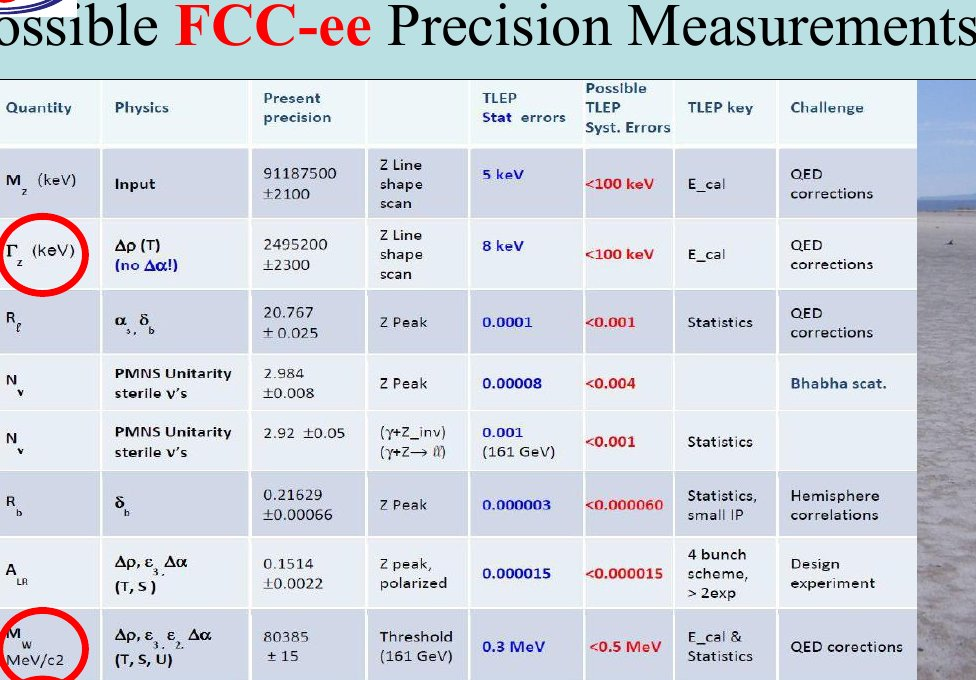
\includegraphics[width=118mm,height=85mm]{JEllis.jpg}}

\end{frame}
%----------------------------------------------------------------------

%----------------------------------------------------------------------
\begin{frame}[fragile]
\frametitle{\bf Lesson from LEP. {\yel Three golden rules} }

\bf
From LEP experience we know that\\
for the successful mastering of the QED correction effects\\
three criteria has to be met SIMULTANEOUSLY:
\begin{enumerate}
\item\cbl
Resummation of soft photons, collinear mass logarithms to $\infty$ order,\\
AND exploit RGE, $(\Gamma/M)$ and $(t/s)$, suppressions etc.
\item\cmg
Inclusion of the SELECTED higher order Feynman diagrams,
\item\crd
Monte Carlo event generator implementation
\end{enumerate}


\end{frame}
%----------------------------------------------------------------------


%----------------------------------------------------------------------
\begin{frame}[fragile]
\frametitle{\bf {\yel The example of QED Precision time evolution}\\
 in the project where {\yel 3 golden rules} are followed}

\vspace{-2mm}
{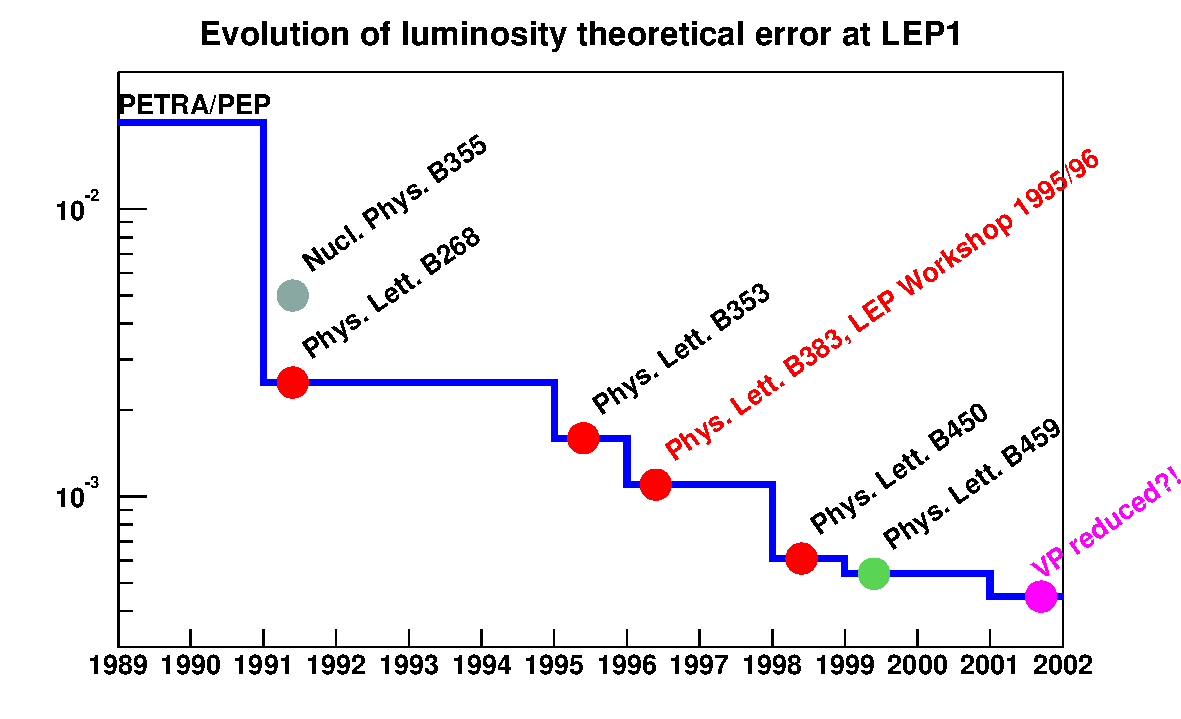
\includegraphics[width=110mm,height=80mm]{cFigA.pdf}}

\end{frame}
%----------------------------------------------------------------------


%----------------------------------------------------------------------
\begin{frame}[fragile]
\frametitle{\bf Not only photonic corrs.! Watch out for Vac.Pol.!}
\framesubtitle{\bf Room of improvement by {\yel factor 2-4} exists but... 
 (TP=Technical Precision)}

\vspace{-2mm}
{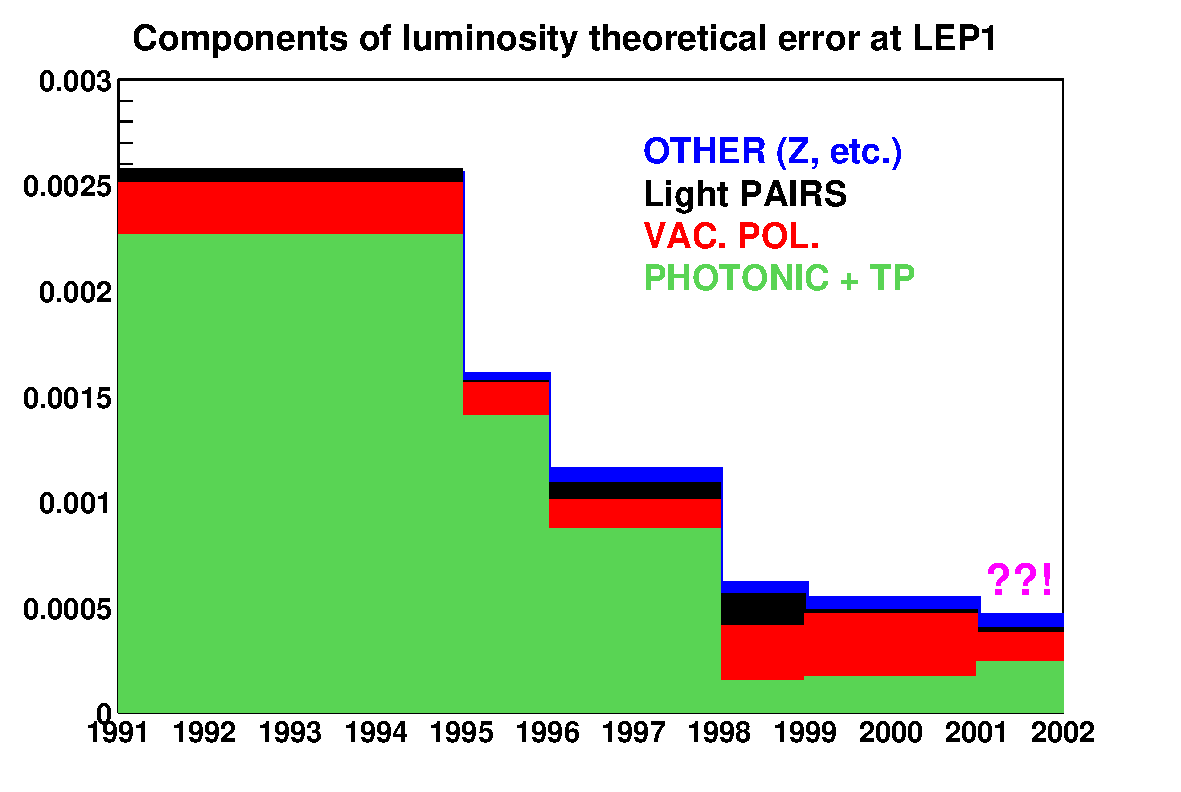
\includegraphics[width=110mm,height=80mm]{cFigB.pdf}}

\end{frame}
%----------------------------------------------------------------------

%----------------------------------------------------------------------
\begin{frame}[fragile]
\frametitle{\bf Progress after LEP?}

\bf
My personal impressions on the progress in QED corr. calculations after LEP:
\begin{itemize}
\item
Enormous progress in last 12 years, in the methods
for h.o. calculations of multiloop and multileg calculations,
for ILC and LHC processes!!!
\item
Unfortunately, they are often not in a form suitable for matching
with the QED soft/collinear resummation.
\item
In the MC codes for the QED corrs. for FCC-ee, essentially,
there is (almost) nothing new/better than at the end of the LEP era
\item
Let's make catalogue of these codes, as
they could be used for various studies 
and should serve as a starting point for the future developments.
\item
It is easy for me, as they come mostly from my own Krakow group:))
\end{itemize}

\end{frame}
%----------------------------------------------------------------------


%----------------------------------------------------------------------
\begin{frame}[fragile]
\frametitle{\bf LEP MC programs from Krakow group}
\framesubtitle{\bf with the important US component: B.F.L Ward, S.Yost!}

Contact persons will tell you where to look for source code
which compiles under modern Linux:
\begin{itemize}
\item
{\cbl\bf KKMC} for $e^-e^+ \to f\bar{f}+ n\gamma$,\\
$f=\mu,\tau,\nu,u,d,s,c,b$,~~~~ $n=0,1,2...\infty$\\
{\em contact: S. Jadach, stanislaw.jadach$@$cern.ch}
\item
{\cbl\bf TAUOLA} for $\tau$ decays and
{\cbl\bf PHOTOS} for extra photons emission
$\in$ KKMC and other programs, including LHC!\\
{\em contact: Z. W{\c a}s, zbigniew.was$@$cern.ch}
\item
{\cbl\bf BHLUMI} for small angle $e^-e^+ \to e^-e^+$\\
{\em contact: S. Jadach, stanislaw.jadach$@$cern.ch}
\item
{\cbl\bf BHWIDE} for large angle $e^-e^+ \to e^-e^+$\\
{\em contact: W. P\l{}aczek, wieslaw.placzek$@$uj.edu.pl}
\item
{\cbl\bf KORALW} for $e^-e^+ \to 4f $,
{\cbl\bf YFSWW} $e^-e^+ \to W^-W^+ \to 4f $\\
{\em contact: M. Skrzypek, maciej.skrzypek$@$ifj.edu.pl}
\item
{\cbl\bf YFSZZ} for $e^-e^+ \to ZZ \to 4f $\\
{\em contact: W. P\l{}aczek, wieslaw.placzek$@$uj.edu.pl}
\end{itemize}

\end{frame}
%----------------------------------------------------------------------


%----------------------------------------------------------------------
\begin{frame}[fragile]
\frametitle{\bf More on KKMC}

\bf\Large
Due to limited time,\\
let me say a few more words on KKMC,\\
finishing with small example\\
of new study on QED uncertainty estimate\\
in \fbox{$N_\nu \in \nu\bar\nu\gamma$} using KKMC.

\end{frame}
%----------------------------------------------------------------------

%----------------------------------------------------------------------
\begin{frame}[fragile]
\frametitle{\bf What is KKMC?}
{\large
KKMC is the MC event generator for the process:\\
~~~~~~~~~~~~~~\fbox{\cbl $e^-e^+ \to f\bar{f}+ n\gamma$}\\
{\cbl $f=\mu,\tau,\nu,u,d,s,c,b$,~~~~ $n=0,1,2...\infty$.}
}\\
Interfaced with TAUOLA+PHOTOS\\
and interfaced with electroweak library DIZET.\\

Published version \fbox{\cmg 4.13} (to be cited):
\begin{itemize}
\item
Comput.Phys.Commun. 130(2000) 360, hep-ph/9912214,\\
F77 code description and user guide (manual).
\item
Phys. Rev. D63 (2001) 113009, hep-ph/0006359\\
physics content, CEEX exponentiation of QED corrs.\\
\end{itemize}
"Workhorse" in data analysis of all four LEP collaborations.\\
~~~\\
\footnotesize
(Replacement of earlier MC's KORALZ and KORALB.)\\
(Not applicable for  $e^-e^+ \to e^-e^+$)

\end{frame}
%----------------------------------------------------------------------

%----------------------------------------------------------------------
\begin{frame}[fragile]
\frametitle{\bf More KKMC versions available since 2000}
\framesubtitle{http://jadach.web.cern.ch/jadach/KKindex.html}
\small
\begin{itemize}
\item
Production Version \fbox{\cmg 4.16}, Oct. 2001,  
(KKMC-v.4.16d-export.tar.gz).
{\cbl Improved $\nu\bar{\nu}$ matrix elm.}\\
RRes module for $\gamma^* \to narrow~resonances$ at LEP.
\item
Developement Version \fbox{\cmg 4.19}, Sept. 2002,  
(KKMC-v.4.19.b-export.tar.gz). {\cbl With C++ wrappers.}\\
Improved $\nu\bar{\nu}$ matrix element and RRes for low energy colliders.\\
ISR with complete NLO corrs,
as in Phys.Rev. D65(2002) 073030 by S.J., M.Melles, B.F.L.Ward and S.A. Yost.\\
{\cbl Collinear beamstrahlung} for NLC/ILC.
\item
Developement Version \fbox{\cmg 4.22}, June 2013,  
(KKMC\_v4\_22.tgz).
Tested with {\cbl $\mu^-\mu+$ and $q\bar{q}$ beams}
(instead of $e^-e^+$) at fixed energy.
Optionally, collinear PDFs for $q\bar{q}$ beams instead of beamstrahlung,
as a patch in the source code (temp. solution).
\item
{\footnotesize
The complete "algebraic" description of the {\cbl QED NNLO} formulas has been
published in Phys.Rev. D73 (2006) 073001
(an extension of the work in Phys.Rev. D65 (2002) 073030),
the code still not public.\\
PHOKHARA MC is an alternative here for low energy colliders.}
\end{itemize}

\end{frame}
%----------------------------------------------------------------------

%----------------------------------------------------------------------
\begin{frame}[fragile]
\frametitle{\small\bf H.O. QED corrs. estimate
 in $e^-e^+\to\nu+\bar\nu+\gamma$, for $N_\nu$ measurement}
\framesubtitle{Study using KKMC: CEEX2 versus CEEX1}

\vspace{-2mm}
{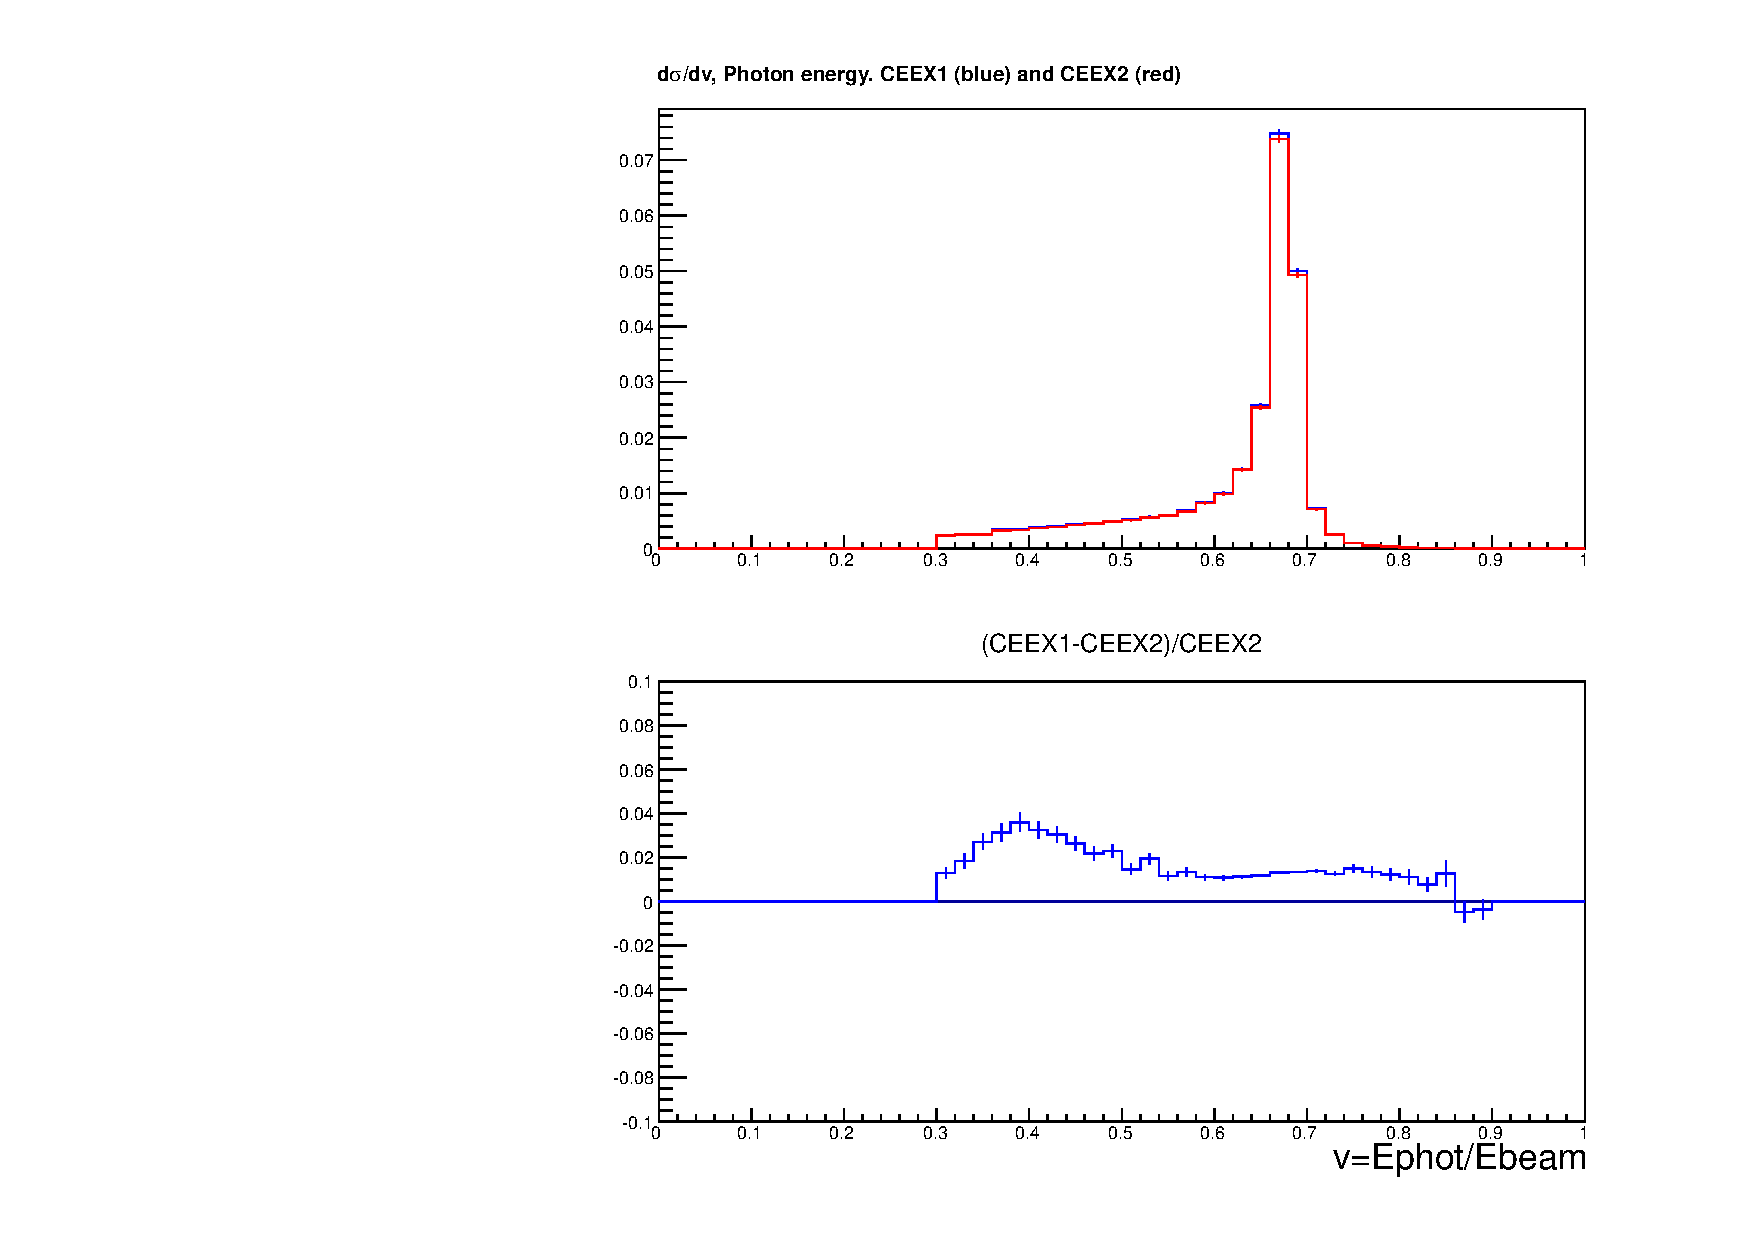
\includegraphics[width=80mm,height=55mm]{mcCeex21.pdf}}

\footnotesize
Min. photon angle $\Theta_{\min}=15^o$,\\
Min. photon energy $x_\gamma=0.3$, ~~~$E_\gamma > x_\gamma E_{beam}$,\\
Min. phot. transv. mom. $x_T=0.3$, ~~~$k^T_\gamma > x_\gamma E_{beam}$,\\
Only one photon within the above restrictions.

\footnotesize
CEEX1= Born +soft photon resum.,
CEEX2= 1st ord. +soft photon resum.

{\crd $\sim$ 2\% effect is seen!}

\end{frame}
%----------------------------------------------------------------------


%----------------------------------------------------------------------
\begin{frame}[fragile]
\frametitle{\bf Sorry about omissions due to limeted time/scope!}
For example I would tell you more about:
\begin{itemize}
\item
Other usefull MC codes from LEP era and some of the extedend
for NLC/ILC like for $ee\to 4f\gamma$ 
RacoonWW by S.Dittmaier and A.Denner, WPHACT by A.Bellestrero,
WHIZARD by T. Ohl, for Bhabha process
SABSPV by O.Nicrosini et.al.
\item
Two-loop Electroweak corrections by several groups
\item
KORALW version in quadri-precision under newest Linux gcc by M. Skrzypek
\item
unpublished scheme of photon resummations near WW threshold by myself
\item
and more...:)
\end{itemize}


\end{frame}
%----------------------------------------------------------------------


%----------------------------------------------------------------------
\begin{frame}[fragile]
\frametitle{\bf Conclusions}

\begin{itemize}
\item
MC codes from LEP era are still defining
the state of art for QED correction FCC-ee.
\item
Most of legacy codes are maintained under present compilers/systems.
\item
One may contact their main authors for more info.
\item
Certain things in the were done better than needed
for LEP, and may be useful for FCCee.
\end{itemize}

\end{frame}
%----------------------------------------------------------------------


%%%%%%%%%%%%%%%%%%%%%%%%%%%%%%%%%%%%%%%%%%%%%%%%%%%%%%%%%%%%%%%%%%%%%%%%%%%
%%%%%%%%%%%%%%%%%%%%%%%%%%%%%%%%%%%%%%%%%%%%%%%%%%%%%%%%%%%%%%%%%%%%%%%%%%%
%%%%%%%%%%%%%%%%%%%%%%%%%%%%%%%%%%%%%%%%%%%%%%%%%%%%%%%%%%%%%%%%%%%%%%%%%%%
%%%%%%%%%%%%%%%%%%%%%%%%%%%%%%%%%%%%%%%%%%%%%%%%%%%%%%%%%%%%%%%%%%%%%%%%%%%



%----------------------------------------------------------------------
\begin{frame}[fragile]
\frametitle{\bf Appendix}

\vspace{20mm}
\Huge\bf~~~~~~~~~~~~ APPENDIX
\end{frame}
%----------------------------------------------------------------------


%----------------------------------------------------------------------
\begin{frame}[fragile]
\frametitle{\bf Main features of KKMC}
%\framesubtitle{Can be useful for LHC?}

KKMC includes some features which were "overkill" for LEP,
which can be exploited for FCCee:
\begin{itemize}
\item
Resummed (exponentiated) multiphoton effects at the amplitude level.\\
About 10 man-years of work in QED:)
\item
QED rad. corrections up to third LO and NLO,
both in the initial and final state
\item
Plus (exponentiated) initial-final QED interferences.
\item
Most sophisticated M.E. for $e^+e^-\to \nu+\bar\nu+2\gamma$,
with t-channel $W$ exchange,
\item
Complete spin effects, longitudinal+transverse(!) correlations, 
for incoming beams and outgoing femions, mandatory for taus.
\item
Interface to external library of Electroweak corrections
\item
beamstrahlung and more...
\end{itemize}
\end{frame}
%----------------------------------------------------------------------

%----------------------------------------------------------------------
\begin{frame}[fragile]
\frametitle{\bf More on KKMC version 4.22 (2013)}
\framesubtitle{\bf\large Technical points}
\small
\begin{itemize}
\item
Old benchmarks, Table III in Phys.Rev. D 63 (2001) and more,
are reproduced under SLC5 and SLC6, 
after adjustments of flags in makefile's
and minor corrections in f77 code.
\item
Unpublished (public) v.4.16,4.19 include varying subset of extra subdirectories,
not included in v4.13. Also not in v.4.22.
\item
System of original interrelated custom $Makefile$'s 
is renamed $Makefile\to KKMakefile$
and preserved.
\item
$Automake/Autotools$ are introduced ($makefile.am$ etc.).\\
Hence KKMC is more platform independent\\
and can be easily put under $kdevelop3$ or $eclipse$.
\item
Interface to C++ is provided.
Main program (histogramming, etc) can be in C++, using optionally ROOT.
(On request, or in v4.19)
\item
Scripts for running on PC-farms slightly upgraded and working.
\item
Old versions of PHOTOS and TAUOLA.
\end{itemize}
\end{frame}
%----------------------------------------------------------------------



\end{document}
%%%%%%%%%%%%%%%%%%%%%%%%%%%%%%%%%%%%%%%%%%%%%%%%%%%%%%%%%%%%%%%%%%%%%%%%
%%%%%%%%%%%%%%%%%%%%%%%%%%%%%%%%%%%%%%%%%%%%%%%%%%%%%%%%%%%%%%%%%%%%%%%%
%%%%%%%%%%%%%%%%%%%%%%%%%%%%%%%%%%%%%%%%%%%%%%%%%%%%%%%%%%%%%%%%%%%%%%%%
%%%%%%%%%%%%%%%%%%%%%%%%%%%%%%%%%%%%%%%%%%%%%%%%%%%%%%%%%%%%%%%%%%%%%%%%


%----------------------------------------------------------------------
\begin{frame}[fragile]
\frametitle{Abstract (plan of the talk)}
%\framesubtitle{Mission statement}
...
\end{frame}
%----------------------------------------------------------------------


